\documentclass[12pt]{article}
\usepackage[utf8]{inputenc}
\usepackage{amsmath,amssymb,amsthm}
\usepackage[danish,british]{babel}
\usepackage[pdftex]{graphicx}
\usepackage{pdfpages}
\usepackage{listings}
\usepackage{pgf}
\usepackage{verbatim}
\usepackage{hyperref}
\usepackage{float}

\usepackage{xcolor}

\definecolor{secnum}{RGB}{102,102,102} 

\makeatletter
    \def\@seccntformat#1{\llap{\color{secnum}\csname the#1\endcsname\hskip 16pt}}
\makeatother
\date{}
\title{Tablet Guide}

\begin{document}
\pagenumbering{arabic}
\maketitle
\begin{center}
*Flot billede!*\\
WOW DET ER SMUKT
\end{center}


\newpage
\section{Knapper}
\begin{figure}[H]
  \centering
  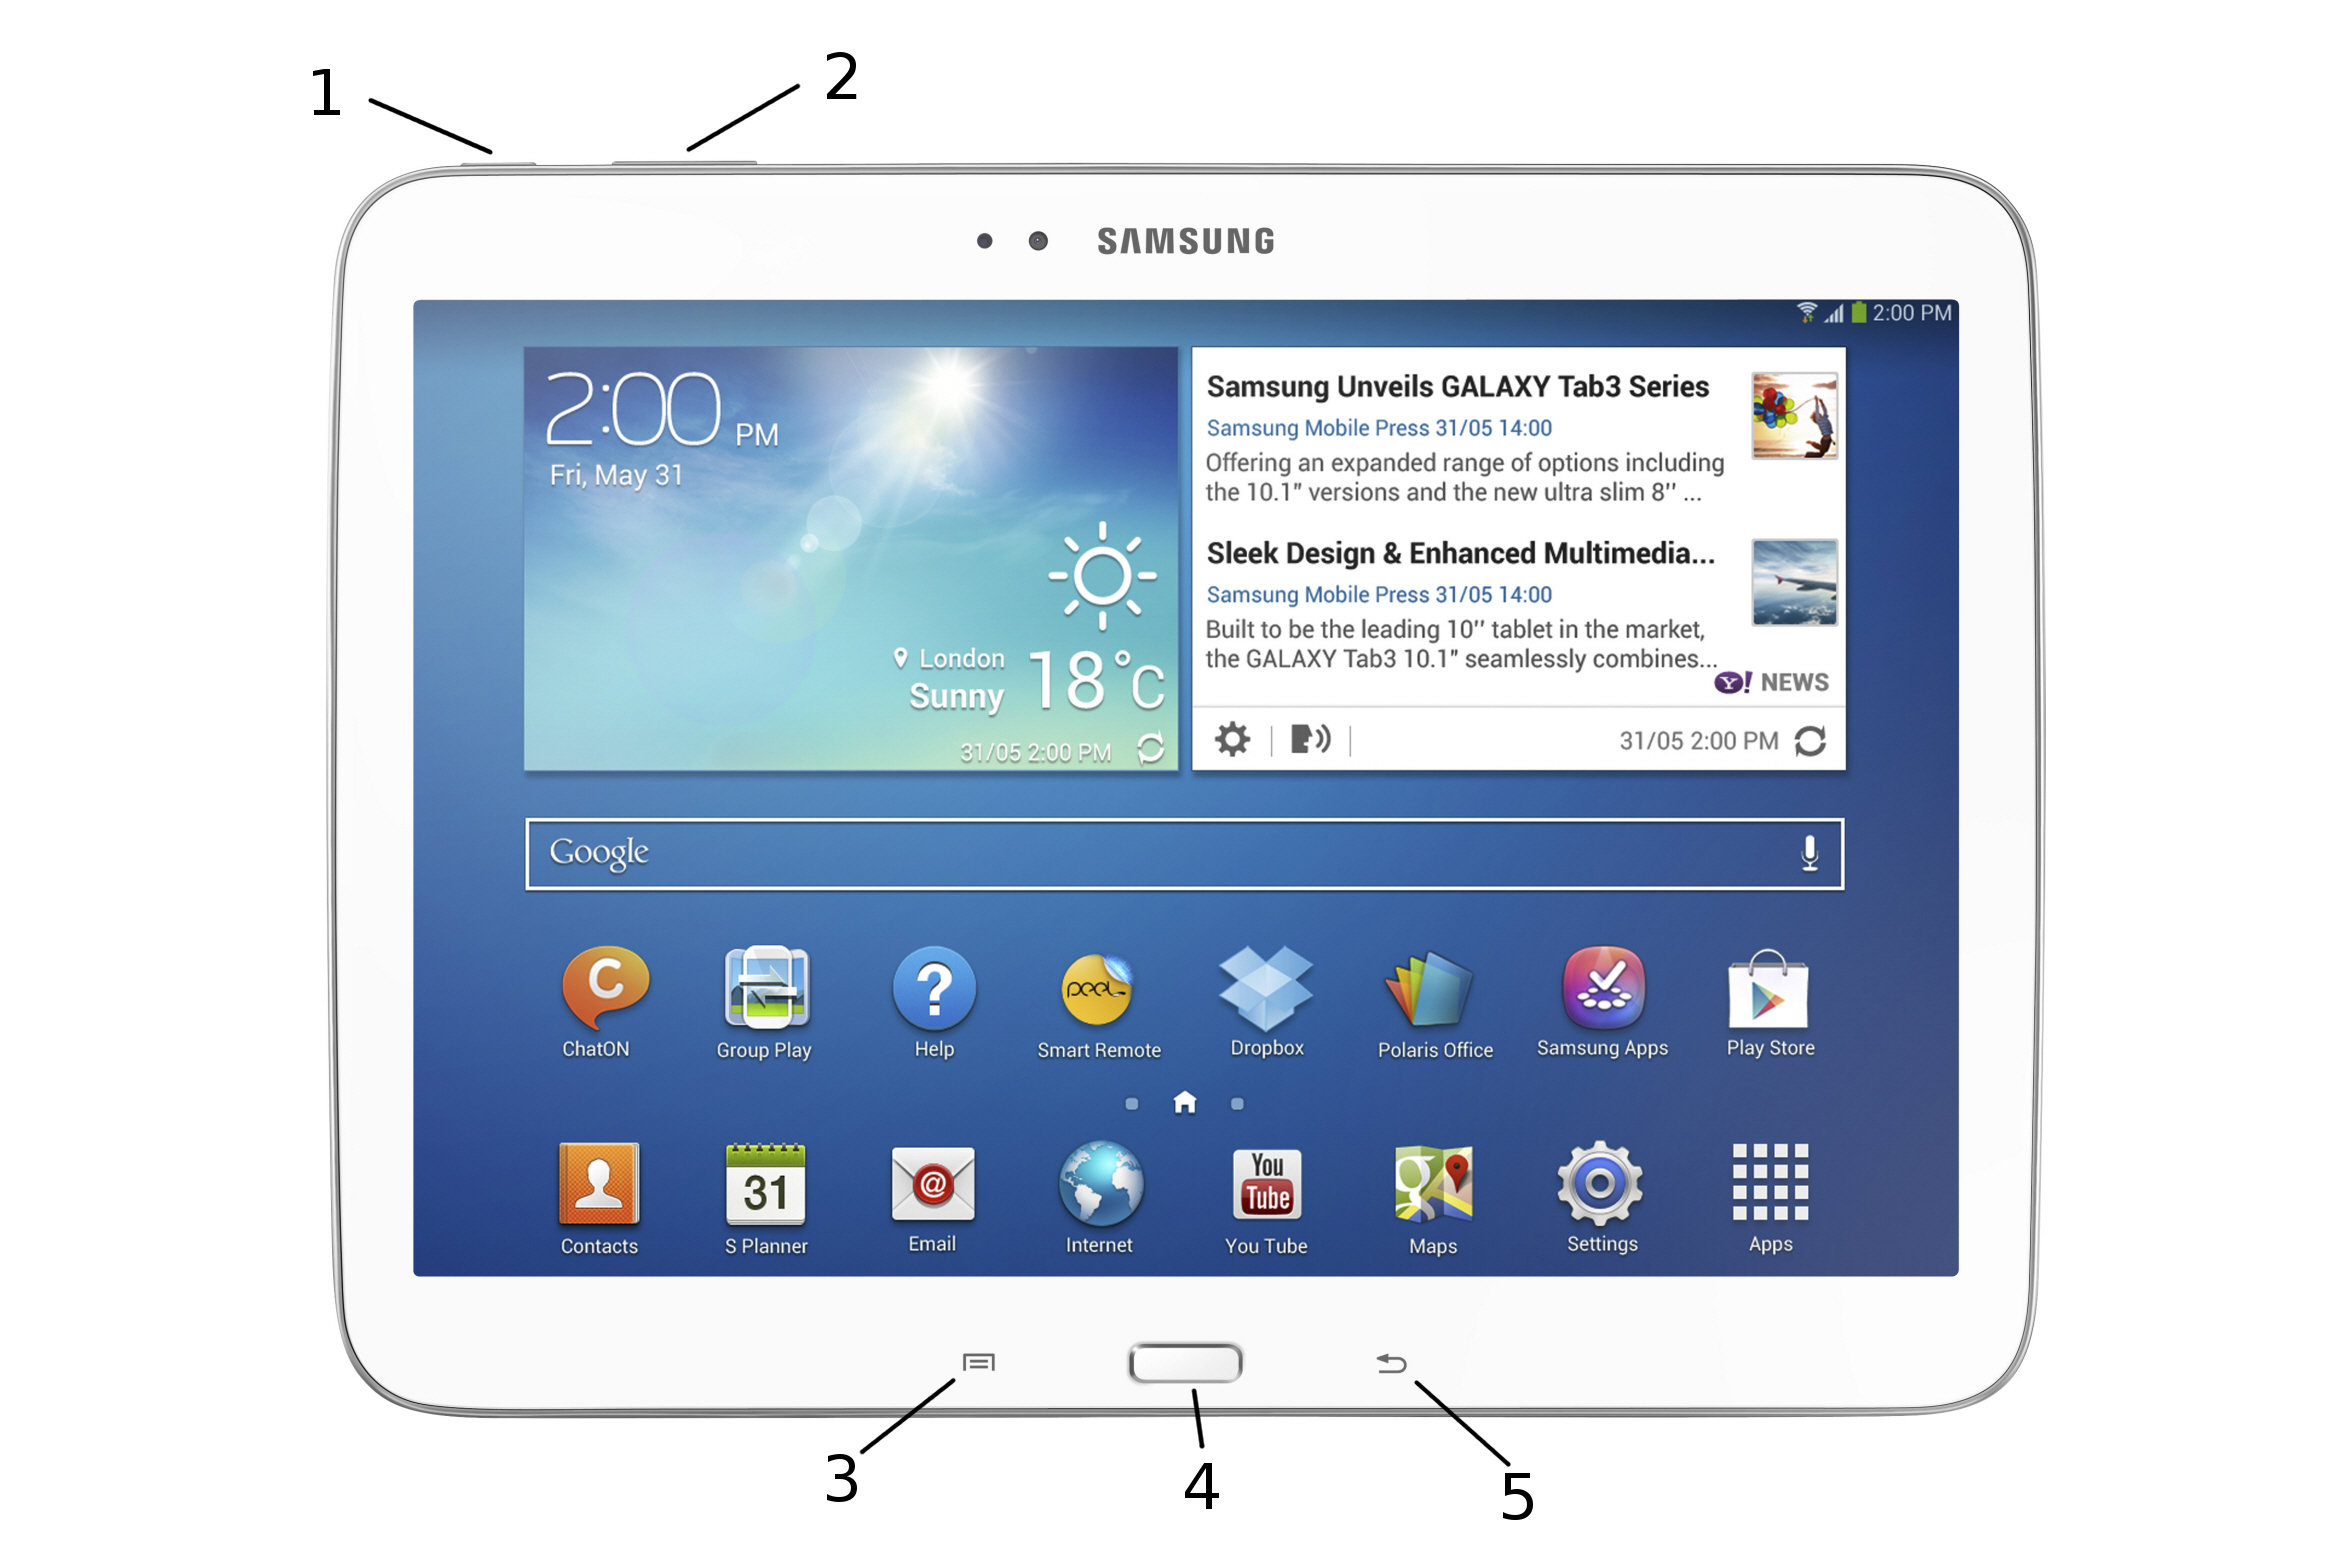
\includegraphics[width=1.0\textwidth]{knapper.jpg}
  \caption{Knapper}
  \label{fig:knapper}
\end{figure}

\begin{enumerate}
    \item Tænd og sluk knap. Et lang tryk tænder den, hvis den er slukket og
        slukker den, hvis den er tændt. Et kort tryk låser skærmen.
    \item Lydjustering. Knappen er følsom i begger ender, og justerer lyden
        op eller ned alt efter, hvilken man trykker på.
    \item Viser åbne programmer. 
    \item Bringer dig til forsiden.
    \item Går et trin tilbage.
\end{enumerate}

\newpage
\section{Forsiden}
\begin{figure}[H]
  \centering
  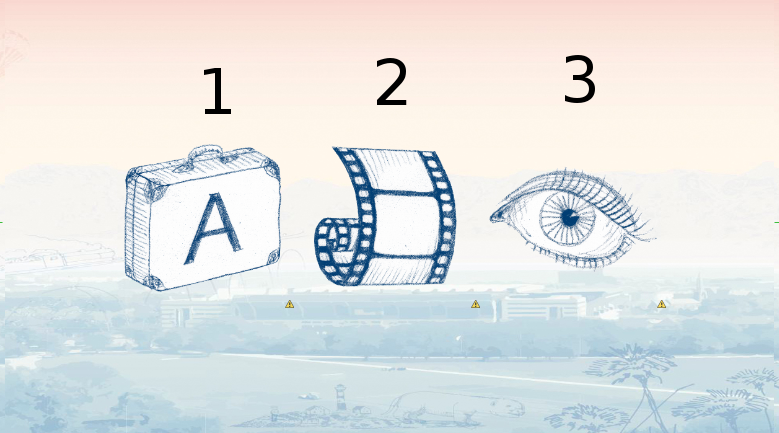
\includegraphics[width=1.0\textwidth]{forside.png}
  \caption{Forsiden består af 3 knapper}
  \label{fig:forside}
\end{figure}

\begin{enumerate}
    \item Går til installerede applikationer.
    \item Går til film.
    \item Går til "opdagelse i gangen".
\end{enumerate}

\newpage

\section{Undersider}
\subsection{Applikationer (Kufferten med A'et)}
På applikationssiden er der 5 billeder, som alle starter et program ved tryk.

\subsection{Film (Filmstriben)}
På film siden er der 5 billeder med en tilhørende aldersgruppe. Ved tryk på et
af disse, kommer man til en liste af film tilhørende den valgte aldersgruppe.
Disse kan alle afspilles ved et enkelt tryk.

\subsection{Opdagelse (Øjet)} 

Indeholder noget inspirerende tekst og nederst en applikation, som brugerne
kan lave deres egen historie med.

\newpage
\section{Fejlfinding}
\subsection{Trinvis guide}
\begin{itemize}
    \item Der er en underlig menu på skærmen, som brugeren ikke kan komme væk
        fra.
        \begin{enumerate}
            \item Tryk på den store knap under skærmen (startknappen)
        \end{enumerate}
    \item Billedet vender når man drejer skærmen.
        \begin{enumerate}
            \item Nogen er kommet til at slå skærmlåsen fra.
            \item For at løse dette skal indstillinger åbnes.
            \item Placer fingeren i toppen af skærmen (Der er en tynd sort
                streg)
            \item Træk fingeren ned af skærmen til indstillingsmenuen er
                tydeligt fremme.
            \item Hvis "Skærm rotation" lyser grønt, så tryk på denne for at
                slå den fra.
            \item Tryk på startknappen for at lukke indstillinger igen.
        \end{enumerate}
\end{itemize}

\subsection{Kontakt}

Hvis du stadig har problemer, og kollegaer ikke kan hjælpe, så skriv en
email til Lasse Ahlbech Madsen (dreadmuffin@gmail.com), hvor du beskriver
problemet.

\end{document}
